\chapter{Experimenty}
Po dokončení jsme náš vyhledávač OsmWalk vyzkoušeli na hledání pěších tras po
Praze. Zkoumali jsme rychlost vyhledávání tras, jejich vhodnost a správnost
odhadu času a vzdálenosti. Také jsme prvedli několik měření porovnávající různé
dostupné vyhledávače cest.

Každá porovnávaná trasa obsahuje popis, obrázek ukazující nalezené cesty
jednotlivých vyhledávačů a srovnání parametrů nalezených cest. Položka {\it
Vlastní měření} je naměřený čas a vzdálenost při chůzi po trase nalezené naším
vyhledávačem. Na obrázcích, využívajících mapové podklady OSM, jsou jednotlivým
vyhledávačům přiřazeny následující barvy:
\begin{itemize}
\item zelená -- náš vyhledávač OsmWalk
\item modrá -- Mapy.cz
\item červená -- Google Maps
\item fialová -- OsmAnd
\end{itemize}

\section{Trasa středem města}
Trasa vedoucí od Čertovky na Florenc. Trasa prochází středem města, což je hustá
zástavba bez větších volných ploch. Většina území je pěší zóna, tudíž nejsou
problémy se špatnou návazností chodníků v~mapových podkladech. Vylepšení našeho
vyhledávače v~podobě spojek ani zkratek by zde nemělo hrát velkou roli.
\begin{figure}[h]
	\centering
	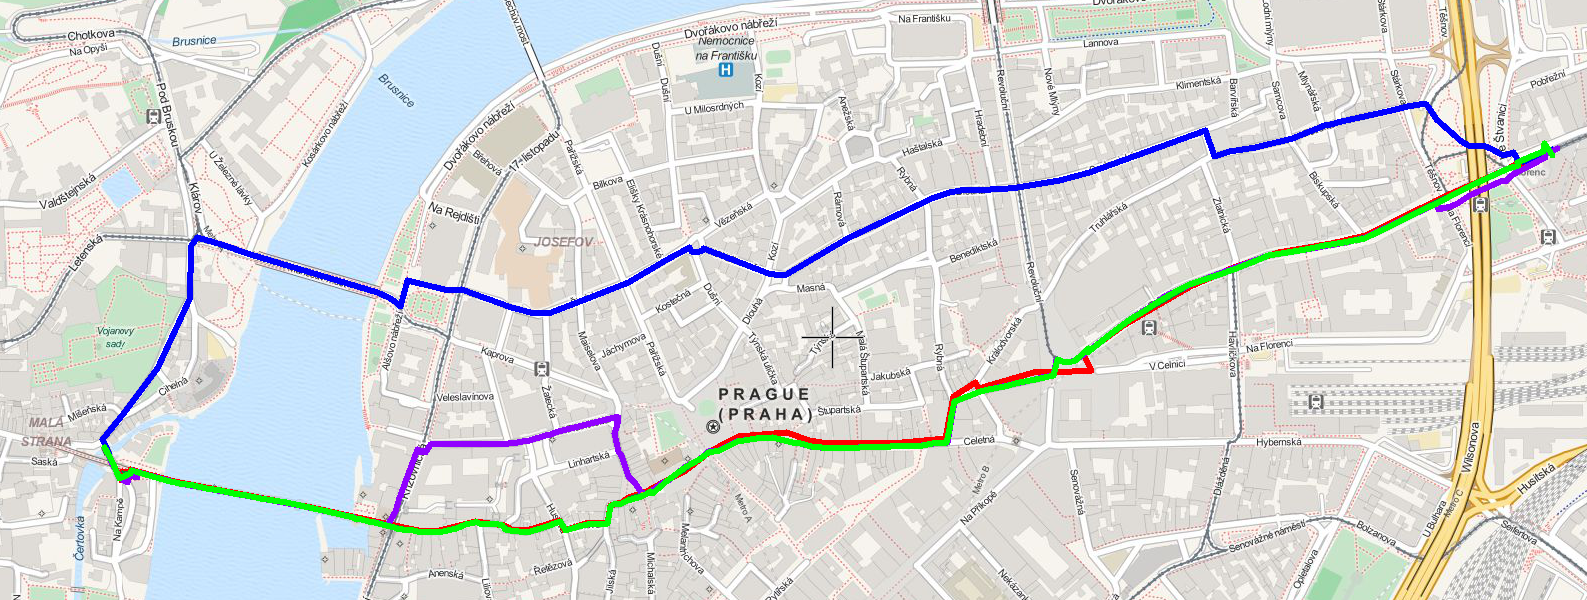
\includegraphics[width=13cm]{../img/km-frc.png}
	\caption{Trasa přes střed města}
	\label{fig:km-frc}
\end{figure}
\begin{itemize}
	\item OsmWalk: 2.5\,km, 25\,min
	\item Mapy.cz: 2.7\,km, 40\,min
	\item Google maps: 2.5\,km, 31\,min
	\item OsmAnd: 2.6\,km, 30\,min
	\item Vlastní měření: 2.5\,km, 26\,min
\end{itemize}
Nalezené trasy (viz obr. \ref{fig:km-frc}) byly přibližně stejně dlouhé a kromě Map.cz se lišily jen
minimálně. Čas Map.cz se s~ohledem na délku jevil jako přemrštěný, odhad délky a
času našeho vyhledávače byl přesný. 


\section{Trasa přes most Barikádníků}
Trasa vedoucí z~kolejí 17.~listopadu na autobusovou zastávku Nádraží Holešovice.
Na této trase je podstatné, že hledáme trasu pro pěší a nechceme chodit po
šestiproudé magistrále. Optimální cesta používaná studenty kolejí obsahuje
několik pěšin, které nemusí být dobře zmapovány, tudíž zde je možnost využití
spojek a zkratek.

\begin{figure}[h]
	\centering
	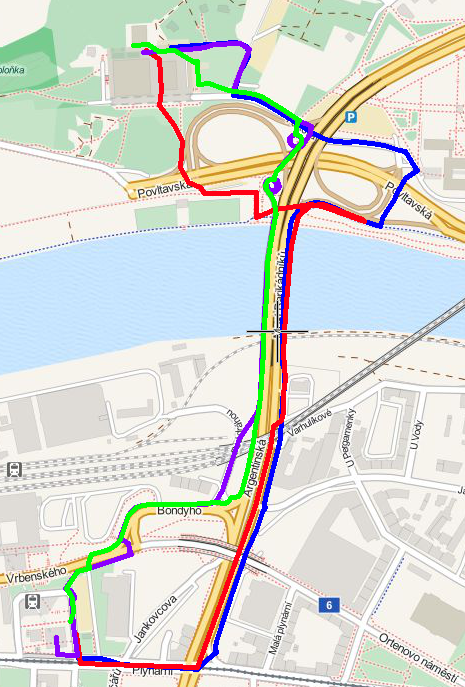
\includegraphics[width=13cm]{../img/kol-hol.png}
	\caption{Trasa přes most Barikádníků}
	\label{fig:kol-hol}
\end{figure}

\begin{itemize}
	\item OsmWalk: 1.3\,km, 14\,min
	\item Mapy.cz: 1.7\,km, 26\,min
	\item Google maps: 1.6\,km, 22\,min
	\item OsmAnd: 1.6\,km, 21\,min
	\item Vlastní měření: 1.3\,km, 13\,min
\end{itemize}
Trasy nalezené jednotlivými vyhledávači (viz obr. \ref{fig:kol-hol}) se zde výrazně lišily. Podrobnější
zkoumání ukázalo, že ani Mapy.cz ani Google Maps neumí správně používat podchod
pod ulicí Povltavská. Tyto vyhledávače také přešly z~chodníku na silnici,
Mapy.cz v~místě, kdy už po obou stranách silnice vede chodník, Google Maps už
dříve, v~místě, kde vede chodník odděleně od silnice. Naproti tomu OsmAnd našel
trasu zcela korektně po chodnících a uměl i správně použít podchod. Náš
vyhledávač našel téměř optimální trasu, problém mu dělaly rampy z~podchodu na
most. Na konci naplánoval trasu po spojce mimo přechod, což ale není vadou.
Naměřená skutečná vzdálenost i čas odpovídaly odhadům našeho vyhledávače.

\section{Trasa přes Petřín}
Trasa vedoucí z~Malostranského náměstí na koleje Strahov. Převážná část této
trasy vede přes petřínský park, tudíž je zde potenciál pro využití zkratek. 

\begin{figure}[h]
	\centering
	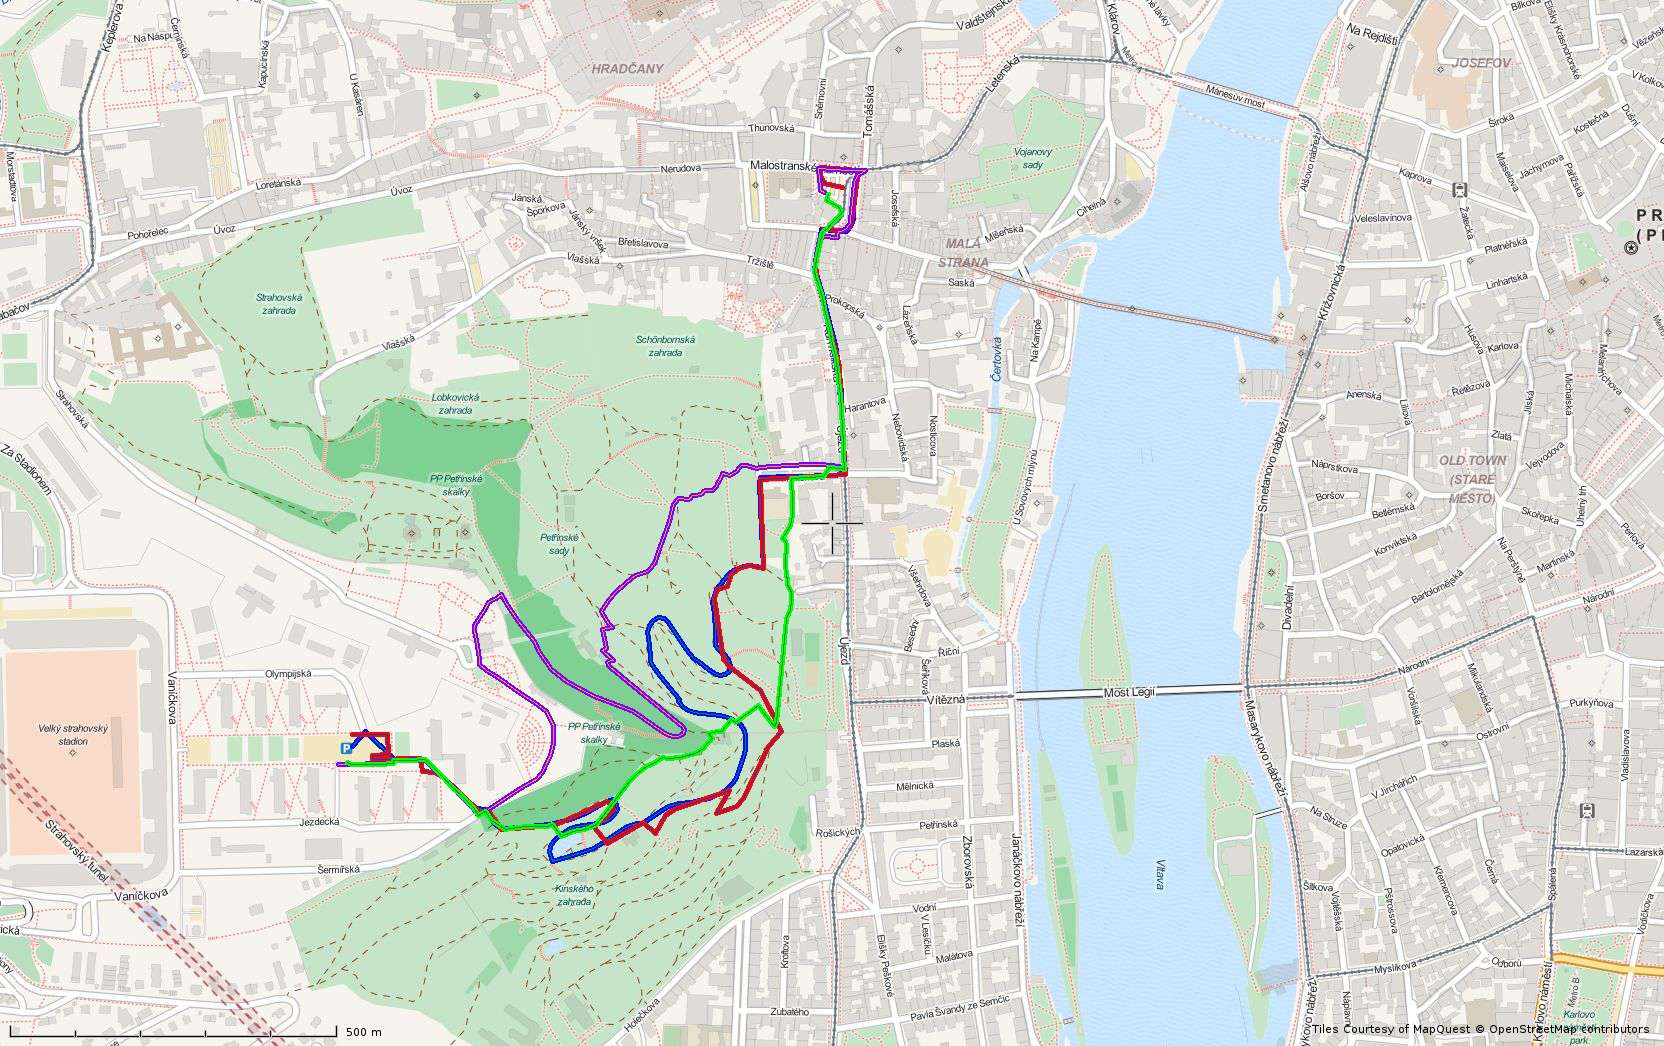
\includegraphics[width=13cm]{../img/ms-sh.png}
	\caption{Trasa přes Petřín}
	\label{fig:ms-sh}
\end{figure}
\begin{itemize}
	\item OsmWalk: 1.7\,km, 25\,min
	\item Mapy.cz: 2.4\,km, 36\,min
	\item Google maps: 2.2\,km, 33\,min
	\item OsmAnd: 2.4\,km, 28\,min
	\item Vlastní měření: 1.8\,km, 21\,min
\end{itemize}

Nalezené trasy (viz obr. \ref{fig:ms-sh}) se lišily využívanými cestami v~Petřínském parku. Náš vyhledávač
využil na cestě několik zkratek, díky čemuž nalezl výrazně kratší trasu. Při
ověřování nalezené trasy jsme zjistili, že by bylo vhodné do vyhledávače přidat
penalizaci za sklon svahu, protože některé zkratky byly téměř neschůdné
pro sklon svahu. I~přes tutuo skutečnost byl čas odhadnutý naším vyhledávačem
mírně nadhodnocený, avšak nejpřesnější. Délka byla odhadnuta přesně.

Experimenty prokázaly, že náš vyhledávač poskytuje z~porovnávaných nejpřesnější
odhady skutečné délky a času nalezených tras. Trasy nalezené vyhledávačem jsou
prakticky použitelné, na místech s~prudkými svahy je potřeba nepoužívat zkratky
nebo upravit vyhledávač, aby uvažoval sklon svahu. 
